\documentclass[aspectratio=169]{beamer}

\usetheme{Madrid}
\usecolortheme{default}
\usefonttheme{serif}
\setbeamertemplate{navigation symbols}{}

\usepackage{amsmath}
\usepackage{amssymb}
\usepackage{graphicx}
\usepackage{iftex}
\usepackage{tikz}
\usetikzlibrary{arrows.meta,positioning}

\ifPDFTeX
  \usepackage{newtxtext}
  \usepackage{newtxmath}
\else
  \usepackage{fontspec}
  \setmainfont{Times New Roman}
  \setsansfont{Times New Roman}
  \setmonofont{Times New Roman}
\fi

\setbeamerfont{normal text}{family=\rmfamily,series=\mdseries}
\setbeamerfont{structure}{family=\rmfamily,series=\mdseries}
\setbeamerfont{frametitle}{family=\rmfamily,series=\mdseries}
\setbeamerfont{title}{family=\rmfamily,series=\mdseries}
\setbeamerfont{itemize/enumerate body}{family=\rmfamily,series=\mdseries}
\setbeamerfont{itemize/enumerate subbody}{family=\rmfamily,series=\mdseries}
\linespread{0.95}

\begin{document}

\begin{frame}{Global Planner Overview}
\small
\begin{columns}[T,onlytextwidth]
\begin{column}{0.62\textwidth}
\begin{flushleft}
\textbf{Map graph}\\[0.3em]
The CARLA global planner builds a directed graph from the HD map:
\[
G=(V,E)
\]
\begin{itemize}
\setlength\itemsep{0.3em}
\item $V$: road-segment endpoint nodes
\item $E$: lane-follow edges and lane-change edges
\end{itemize}

\textbf{Initial route}\\[0.3em]
At the beginning of the simulation, the planner finds the shortest path
\[
\pi_{\mathrm{init}}

=
\operatorname{A^*}(x_{\mathrm{ego}},x_{\mathrm{goal}})
\]
from the ego start position to the scenario final destination.
\end{flushleft}
\end{column}

\begin{column}{0.35\textwidth}
Key idea
\begin{itemize}
\setlength\itemsep{0.3em}
\item The graph comes from map topology.
\item A* search is used inside CARLA's \texttt{trace\_route(...)}.
\item Output is a waypoint sequence for the global route.
\item MPC then tracks this route locally.
\end{itemize}
\end{column}
\end{columns}
\end{frame}

\begin{frame}{When Reroute Is Triggered}
\small
\begin{columns}[T,onlytextwidth]
\begin{column}{0.62\textwidth}
\begin{flushleft}
\textbf{Normal start}\\[0.3em]
\begin{itemize}
\setlength\itemsep{0.3em}
\item No hazard is assumed at the beginning.
\item The vehicle first follows the initial route to the final destination.
\end{itemize}

\textbf{Behavior-planner check}\\[0.3em]
The behavior planner reads cooperative messages from \texttt{cp\_message.json}.

\[
\text{decision}=\texttt{reroute}
\]
only if:
\begin{itemize}
\setlength\itemsep{0.3em}
\item a message of type \texttt{lane\_closure} exists
\item the hazard position is on the current route
\item the hazard is ahead of the ego
\end{itemize}

Otherwise, the planner keeps normal behavior such as
\[
\text{decision}=\texttt{lane\_follow}
\]
\end{flushleft}
\end{column}

\begin{column}{0.35\textwidth}
Inputs from the message
\begin{itemize}
\setlength\itemsep{0.3em}
\item hazard position $(x_h,y_h)$
\item road id
\item lane id
\item raw CARLA lane id
\end{itemize}

Purpose
\begin{itemize}
\setlength\itemsep{0.3em}
\item Do not reroute too early.
\item Do not reroute for hazards outside the active route.
\item Reroute only when the current path is actually affected.
\end{itemize}
\end{column}
\end{columns}
\end{frame}

\begin{frame}{How the New Route Is Found}
\small
\begin{columns}[T,onlytextwidth]
\begin{column}{0.62\textwidth}
\begin{flushleft}
\textbf{Step 1}\\[0.3em]
Snap the hazard position from the cooperative message to the nearest driving waypoint.

\textbf{Step 2}\\[0.3em]
Resolve the CARLA graph edge that contains this blocked waypoint.

\textbf{Step 3}\\[0.3em]
Copy the planner graph and make only that blocked edge unavailable:
\[
w(e_h)=\infty
\]

\textbf{Step 4}\\[0.3em]
Run A* again:
\[
\pi_{\mathrm{new}}
=
\operatorname{A^*}_{\,e_h\ \mathrm{blocked}}
(x_{\mathrm{ego}},x_{\mathrm{goal}})
\]

\textbf{Step 5}\\[0.3em]
If a valid route is found and it avoids the hazard, replace the old global route.
\end{flushleft}
\end{column}

\begin{column}{0.35\textwidth}
Why this works
\begin{itemize}
\setlength\itemsep{0.3em}
\item The blocked lane is no longer attractive to A*.
\item If another lane or branch exists, A* uses it.
\item The goal stays the same: scenario final destination.
\end{itemize}

Fallbacks
\begin{itemize}
\setlength\itemsep{0.3em}
\item blocked raw lane
\item segment penalty
\item blocked-point avoidance
\item adjacent ego-lane retry
\end{itemize}
\end{column}
\end{columns}
\end{frame}

\begin{frame}{Before and After Reroute}
\small
\begin{columns}[T,onlytextwidth]
\begin{column}{0.49\textwidth}
\centering
\textbf{Before hazard handling}\\[0.4em]
\resizebox{0.97\textwidth}{!}{
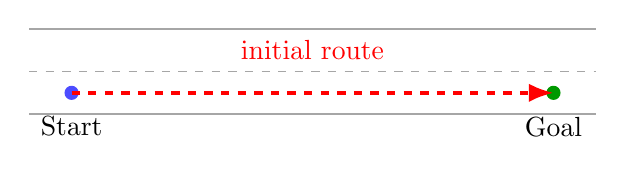
\begin{tikzpicture}[x=0.9cm,y=0.9cm]
  \draw[gray!70, line width=1.0pt] (0,1.2) -- (8,1.2);
  \draw[gray!70, dashed] (0,0.6) -- (8,0.6);
  \draw[gray!70, line width=1.0pt] (0,0.0) -- (8,0.0);

  \fill[blue!70] (0.6,0.3) circle (0.10);
  \node[below] at (0.6,0.1) {Start};

  \fill[green!60!black] (7.4,0.3) circle (0.10);
  \node[below] at (7.4,0.1) {Goal};

  \draw[red, line width=1.3pt, dashed, -Latex] (0.6,0.3) -- (7.4,0.3);
  \node[red] at (4.0,0.9) {initial route};
\end{tikzpicture}
}
\end{column}

\begin{column}{0.49\textwidth}
\centering
\textbf{After lane closure is detected}\\[0.4em]
\resizebox{0.97\textwidth}{!}{
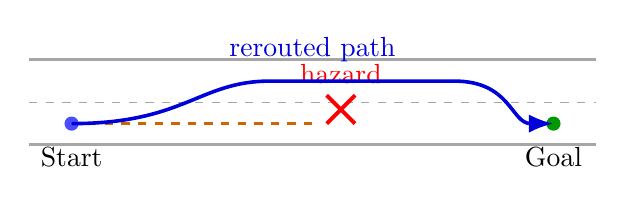
\begin{tikzpicture}[x=0.9cm,y=0.9cm]
  \draw[gray!70, line width=1.0pt] (0,1.2) -- (8,1.2);
  \draw[gray!70, dashed] (0,0.6) -- (8,0.6);
  \draw[gray!70, line width=1.0pt] (0,0.0) -- (8,0.0);

  \fill[blue!70] (0.6,0.3) circle (0.10);
  \node[below] at (0.6,0.1) {Start};

  \fill[green!60!black] (7.4,0.3) circle (0.10);
  \node[below] at (7.4,0.1) {Goal};

  \draw[red, line width=1.4pt] (4.2,0.3) -- (4.6,0.7);
  \draw[red, line width=1.4pt] (4.2,0.7) -- (4.6,0.3);
  \node[red] at (4.4,1.0) {hazard};

  \draw[orange!80!black, line width=1.3pt, dashed] (0.6,0.3) -- (4.0,0.3);
  \draw[blue!85!black, line width=1.3pt, -Latex]
    (0.6,0.3) .. controls (2.2,0.3) and (2.4,0.9) .. (3.4,0.9)
    -- (6.0,0.9)
    .. controls (6.8,0.9) and (6.8,0.3) .. (7.4,0.3);
  \node[blue!85!black] at (4.0,1.35) {rerouted path};
\end{tikzpicture}
}
\end{column}
\end{columns}
\vspace{0.5em}
\begin{itemize}
\setlength\itemsep{0.25em}
\item The old route would pass through the blocked lane.
\item The new route changes lane, bypasses the hazard, and keeps the same goal.
\end{itemize}
\end{frame}

\begin{frame}{Blocked Edge in the Planner Graph}
\small
\begin{columns}[T,onlytextwidth]
\begin{column}{0.52\textwidth}
\centering
\resizebox{0.95\textwidth}{!}{
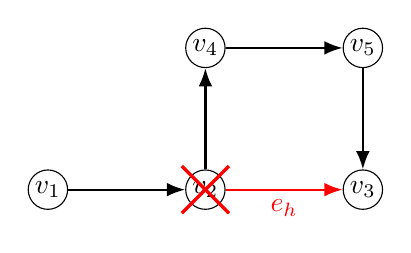
\begin{tikzpicture}[x=1.0cm,y=1.0cm]
  \tikzstyle{vtx}=[circle,draw,minimum size=0.5cm,inner sep=0pt]
  \node[vtx] (a) at (0,0) {$v_1$};
  \node[vtx] (b) at (2,0) {$v_2$};
  \node[vtx] (c) at (4,0) {$v_3$};
  \node[vtx] (d) at (2,1.8) {$v_4$};
  \node[vtx] (e) at (4,1.8) {$v_5$};

  \draw[-Latex,thick] (a) -- (b);
  \draw[-Latex,thick,red] (b) -- node[below] {$e_h$} (c);
  \draw[-Latex,thick] (b) -- (d);
  \draw[-Latex,thick] (d) -- (e);
  \draw[-Latex,thick] (e) -- (c);

  \draw[red, line width=1.2pt] (1.7,-0.3) -- (2.3,0.3);
  \draw[red, line width=1.2pt] (1.7,0.3) -- (2.3,-0.3);
\end{tikzpicture}
}
\end{column}

\begin{column}{0.43\textwidth}
\begin{flushleft}
Graph-based idea
\begin{itemize}
\setlength\itemsep{0.35em}
\item Hazard is snapped to a lane waypoint.
\item The corresponding graph edge is identified.
\item That edge is assigned infinite cost:
\[
w(e_h)=\infty
\]
\item A* then prefers another valid path if one exists.
\end{itemize}
\end{flushleft}
\end{column}
\end{columns}
\end{frame}

\begin{frame}{Why the Previous Reroute Failed}
\small
\begin{columns}[T,onlytextwidth]
\begin{column}{0.49\textwidth}
\begin{flushleft}
\textbf{Previous method}\\[0.3em]
\begin{itemize}
\setlength\itemsep{0.3em}
\item The circles are graph nodes, and the arrows are directed road segments.
\item In this example, the ego and the hazard are both on segment \(s_{eh}\).
\item The old reroute method blocks \(s_{eh}\) and the outgoing links from \(V2\).
\item Then the planner cannot continue from \(V2\) to \(V3\) or \(V4\).
\item So a new route may not be found, even if a local bypass is physically possible.
\end{itemize}

\textbf{Result}\\[0.3em]
\begin{itemize}
\setlength\itemsep{0.3em}
\item no new route found, or
\item the route stays too close to the hazard
\end{itemize}
\end{flushleft}
\end{column}

\begin{column}{0.49\textwidth}
\centering
\textbf{Old planner graph}\\[0.35em]
\resizebox{0.98\textwidth}{!}{
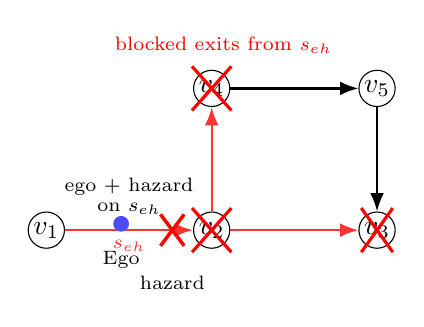
\begin{tikzpicture}[x=1.0cm,y=1.0cm]
  \tikzstyle{vtx}=[circle,draw,minimum size=0.46cm,inner sep=0pt]
  \node[vtx] (a) at (0,0) {$v_1$};
  \node[vtx] (b) at (2.1,0) {$v_2$};
  \node[vtx] (c) at (4.2,0) {$v_3$};
  \node[vtx] (d) at (2.1,1.8) {$v_4$};
  \node[vtx] (e) at (4.2,1.8) {$v_5$};

  \draw[-Latex,thick,red!80] (a) -- node[below] {\scriptsize $s_{eh}$} (b);
  \draw[-Latex,thick,red!80] (b) -- (c);
  \draw[-Latex,thick,red!80] (b) -- (d);
  \draw[-Latex,thick] (d) -- (e);
  \draw[-Latex,thick] (e) -- (c);

  \fill[blue!70] (0.95,0.08) circle (0.10);
  \node[below] at (0.95,-0.15) {\scriptsize Ego};

  \draw[red, line width=1.25pt] (1.45,-0.20) -- (1.75,0.20);
  \draw[red, line width=1.25pt] (1.45,0.20) -- (1.75,-0.20);
  \node[below] at (1.6,-0.46) {\scriptsize hazard};

  \draw[red, line width=1.15pt] (1.85,-0.28) -- (2.35,0.28);
  \draw[red, line width=1.15pt] (1.85,0.28) -- (2.35,-0.28);
  \draw[red, line width=1.15pt] (1.85,1.52) -- (2.35,2.08);
  \draw[red, line width=1.15pt] (1.85,2.08) -- (2.35,1.52);
  \draw[red, line width=1.15pt] (4.0,-0.28) -- (4.4,0.28);
  \draw[red, line width=1.15pt] (4.0,0.28) -- (4.4,-0.28);

  \node[red] at (2.25,2.35) {\scriptsize blocked exits from $s_{eh}$};
  \node at (1.05,0.55) {\scriptsize ego + hazard};
  \node at (1.05,0.27) {\scriptsize on $s_{eh}$};
\end{tikzpicture}
}
\end{column}
\end{columns}

\vspace{0.35em}
\begin{columns}[T,onlytextwidth]
\begin{column}{0.49\textwidth}
\begin{flushleft}
\textbf{Why waypoint A* is better}\\[0.3em]
\begin{itemize}
\setlength\itemsep{0.3em}
\item It checks many nearby waypoints, not only big road pieces.
\item It blocks only the small area around the hazard.
\item It can move a little and then change lane.
\item That is why it works better when the hazard is very close.
\end{itemize}
\end{flushleft}
\end{column}

\begin{column}{0.49\textwidth}
\centering
\textbf{Local waypoint detour}\\[0.35em]
\resizebox{0.98\textwidth}{!}{
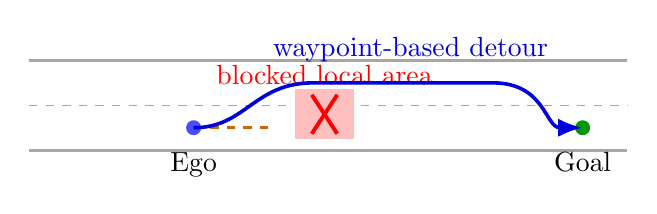
\begin{tikzpicture}[x=0.95cm,y=0.95cm]
  \draw[gray!70, line width=1.0pt] (0,1.2) -- (8,1.2);
  \draw[gray!70, dashed] (0,0.6) -- (8,0.6);
  \draw[gray!70, line width=1.0pt] (0,0.0) -- (8,0.0);

  \fill[blue!70] (2.2,0.3) circle (0.10);
  \node[below] at (2.2,0.1) {Ego};

  \fill[green!60!black] (7.4,0.3) circle (0.10);
  \node[below] at (7.4,0.1) {Goal};

  \fill[red!25] (3.55,0.15) rectangle (4.35,0.82);
  \draw[red, line width=1.4pt] (3.78,0.22) -- (4.12,0.74);
  \draw[red, line width=1.4pt] (3.78,0.74) -- (4.12,0.22);
  \node[red] at (3.95,1.0) {blocked local area};

  \draw[orange!80!black, dashed, line width=1.1pt] (2.2,0.3) -- (3.3,0.3);
  \draw[blue!85!black, line width=1.3pt, -Latex]
    (2.2,0.3) .. controls (2.9,0.3) and (3.0,0.9) .. (3.8,0.9)
    -- (6.2,0.9)
    .. controls (6.9,0.9) and (6.9,0.3) .. (7.4,0.3);
  \node[blue!85!black] at (5.1,1.35) {waypoint-based detour};
\end{tikzpicture}
}
\end{column}
\end{columns}
\end{frame}

\begin{frame}
\small
\begin{flushleft}
\textbf{Previous method}\\[0.3em]
\begin{itemize}
\setlength\itemsep{0.35em}
\item The circles represents graph nodes, and the arrows are directed road segments.
\item When the ego and the hazard are both on the same segment \(V1 \rightarrow V2\).
\item The old reroute method blocked the entire road segment because of a hazard in this segment.
\item Then the planner cannot reach from \(V1\) to \(V2\), even if there is a free lane.
\item So a new route may not be found.
\end{itemize}
\end{flushleft}
\end{frame}

\begin{frame}{Reroute Flowchart}
\centering
\small
\resizebox{0.93\textwidth}{!}{
\begin{tikzpicture}[
  every node/.style={font=\scriptsize},
  node distance=0.55cm and 0.8cm,
  block/.style={
    draw,
    rounded corners,
    align=center,
    minimum width=3.7cm,
    minimum height=0.85cm
  },
  decision/.style={
    draw,
    diamond,
    aspect=2.0,
    align=center,
    inner sep=1pt,
    minimum width=3.6cm,
    minimum height=0.95cm
  },
  line/.style={-Latex,thick}
]
\node[block] (init) {Start simulation};
\node[block,below=of init] (route0) {Initial global route:\\ego $\rightarrow$ final destination};
\node[block,below=of route0] (readmsg) {Read \texttt{cp\_message.json}};
\node[decision,below=of readmsg] (onroute) {Lane closure\\on current route ahead?};
\node[block,below left=0.85cm and 2.2cm of onroute] (follow) {No:\\keep lane follow};
\node[block,below right=0.85cm and 2.2cm of onroute] (snap) {Yes:\\snap hazard to waypoint};
\node[block,below=of snap] (blockedge) {Block hazard graph edge\\by setting cost to $\infty$};
\node[block,below=of blockedge] (astar) {Run A* again:\\ego $\rightarrow$ final destination};
\node[decision,below=of astar] (found) {New route found\\and hazard avoided?};
\node[block,below left=0.85cm and 2.1cm of found] (fallback) {No:\\use fallback reroute methods};
\node[block,below right=0.85cm and 2.1cm of found] (replace) {Yes:\\replace global route};

\draw[line] (init) -- (route0);
\draw[line] (route0) -- (readmsg);
\draw[line] (readmsg) -- (onroute);
\draw[line] (onroute) -- node[left] {No} (follow);
\draw[line] (onroute) -- node[right] {Yes} (snap);
\draw[line] (snap) -- (blockedge);
\draw[line] (blockedge) -- (astar);
\draw[line] (astar) -- (found);
\draw[line] (found) -- node[left] {No} (fallback);
\draw[line] (found) -- node[right] {Yes} (replace);
\end{tikzpicture}
}
\end{frame}

\end{document}
